\subsection{Model tests}
\label{sec:gbi-tests}

\subsubsection{Test 1: Historical walk-forward performance and robustness}
The 36-month trailing-window rolling CVaR policy is the research baseline. It is evaluated on realized monthly returns after quarterly re-optimization with 10bp one-way transaction costs. A fixed Moderate 50/50 benchmark and a frozen policy use the same out-of-sample months. A 48-month rolling result is included only as a window-length sensitivity.

\begin{table}[htbp]
\centering
\footnotesize
\caption{Test 1: Moderate-policy historical walk-forward performance and robustness.}
\label{tab:gbi-historical-robustness}
\begin{tabular}{lrrrrrr}
\toprule
Strategy & Ann. return & Ann. vol. & Sharpe & Max drawdown & ES (95\%) & Months \\
\midrule
36m rolling baseline & 9.11% & 7.38% & 1.22 & -6.85% & 3.61% & 59 \\
36m frozen policy & 9.20% & 9.23% & 1.00 & -14.85% & 5.30% & 59 \\
36m 50/50 benchmark & 9.45% & 9.36% & 1.02 & -14.43% & 4.89% & 59 \\
48m rolling sensitivity & 4.65% & 6.99% & 0.69 & -7.70% & 3.84% & 47 \\
\bottomrule
\end{tabular}
\vspace{2pt}
\begin{minipage}{0.96\linewidth}
\footnotesize
Notes: The 36-month rolling policy is the baseline. The first three rows use the same 59 out-of-sample months, quarterly rebalancing and 10bp one-way transaction costs. The 48-month row is a window-length sensitivity with 47 out-of-sample months. Sharpe assumes a zero risk-free rate.
\end{minipage}
\end{table}


\subsubsection{Test 2: Client-input sensitivity}
This test checks whether personalization inputs create observable changes in the policy recommendation or financial-plan result. The risk scenario changes the selected policy; asset and contribution scenarios change the terminal-wealth assessment; the expense scenario changes the retirement cash-flow gap and priority schedule.

\begin{table}[htbp]
\centering
\scriptsize
\caption{Test 2: client-input sensitivity for the illustrative retirement plan.}
\label{tab:gbi-client-sensitivity}
\begin{tabular}{llrrrrrr}
\toprule
Scenario & Risk & Assets & Contribution & Retirement gap & Projected wealth & Funding & Success \\
\midrule
Base client & Moderate & \$750,000 & \$25,000 & \$32,000 & \$1,216,109 & 105.7% & 66.6% \\
Conservative risk & Conservative & \$750,000 & \$25,000 & \$32,000 & \$1,038,574 & 90.3% & 8.5% \\
Assets -20\% & Moderate & \$600,000 & \$25,000 & \$32,000 & \$1,002,754 & 87.2% & 11.6% \\
Contribution \$15k & Moderate & \$750,000 & \$15,000 & \$32,000 & \$1,156,375 & 100.6% & 48.3% \\
Essential expenses +\$15k & Moderate & \$750,000 & \$25,000 & \$47,000 & \$1,216,109 & 105.7% & 66.6% \\
\bottomrule
\end{tabular}
\vspace{2pt}
\begin{minipage}{0.97\linewidth}
\scriptsize
Notes: All scenarios retain a five-year horizon and a \$1.15 million target. The expense scenario changes the staged retirement cash-flow gap; the current terminal-wealth bootstrap does not yet deduct retirement spending, so its success probability remains unchanged.
\end{minipage}
\end{table}


\begin{figure}[htbp]
  \centering
  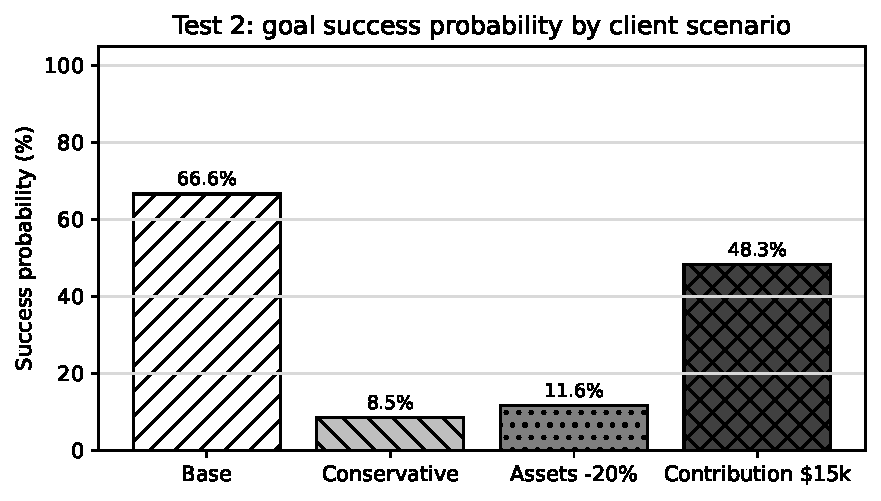
\includegraphics[width=0.82\linewidth]{part2_testing/figures/gbi_client_sensitivity_success_probability.pdf}
  \caption{Historical-bootstrap goal success probability under selected client-input scenarios.}
  \label{fig:gbi-client-sensitivity}
\end{figure}
